\documentclass{standalone}
\usepackage{tikz}
\usetikzlibrary{patterns, positioning}

\begin{document}
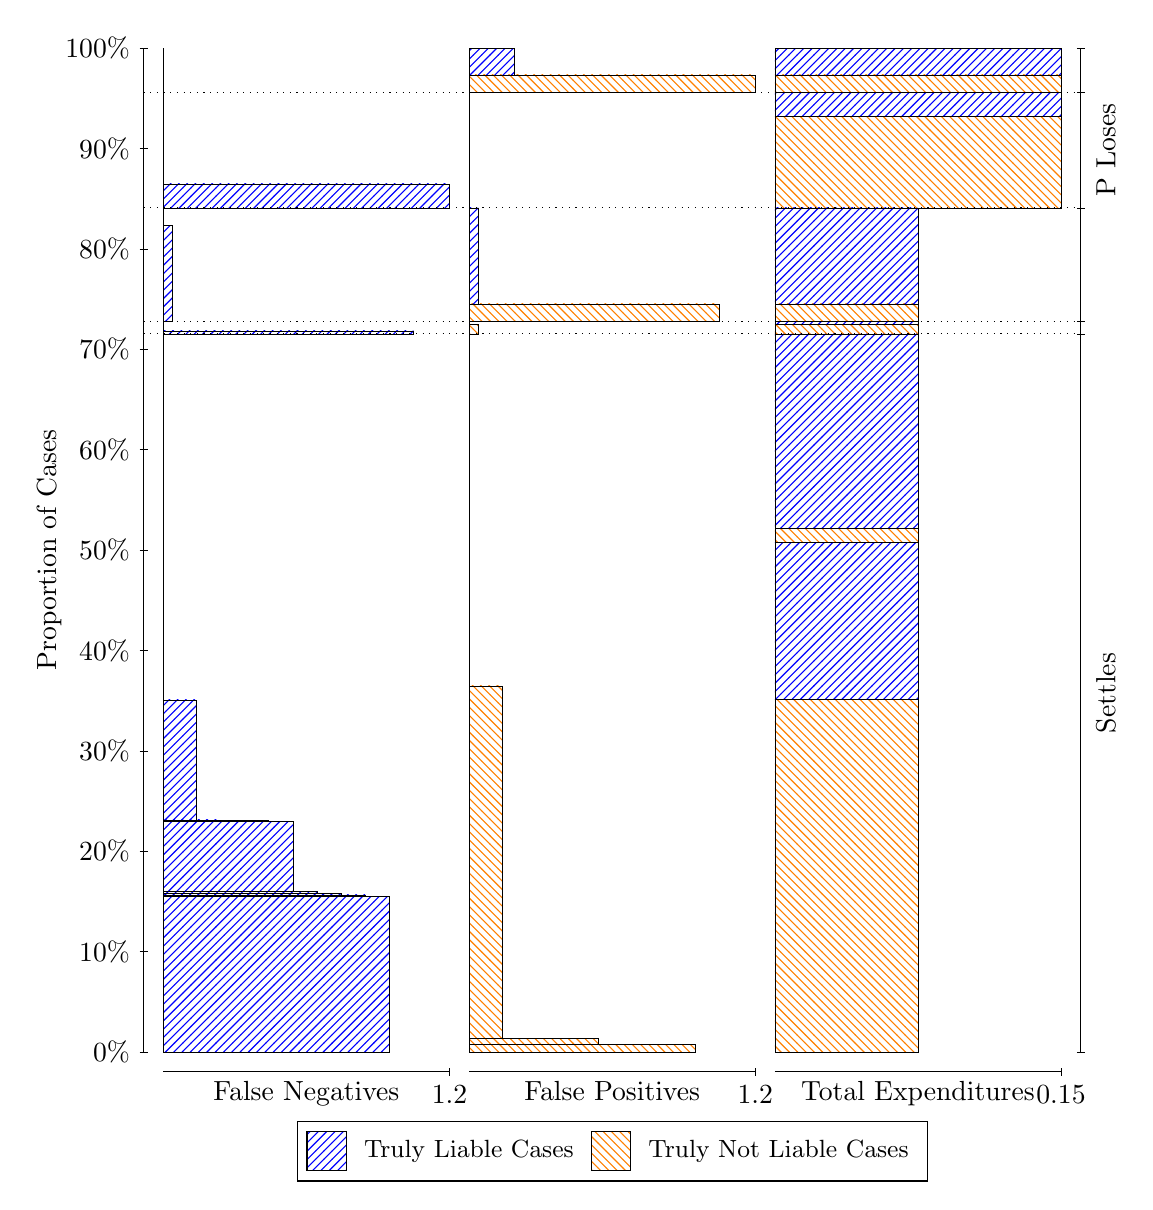
\begin{tikzpicture}
\draw[black, very thin] (1.5,1.75) -- (1.5,14.5);
\node[rotate=90, anchor=center] at (0.3, 8.125) {Proportion of Cases};
\draw[black, very thin] (1.45,1.75) -- (1.55,1.75);
\node[anchor=east] at (1.45, 1.75) {0\%};
\draw[black, very thin] (1.45,3.025) -- (1.55,3.025);
\node[anchor=east] at (1.45, 3.025) {10\%};
\draw[black, very thin] (1.45,4.3) -- (1.55,4.3);
\node[anchor=east] at (1.45, 4.3) {20\%};
\draw[black, very thin] (1.45,5.575) -- (1.55,5.575);
\node[anchor=east] at (1.45, 5.575) {30\%};
\draw[black, very thin] (1.45,6.85) -- (1.55,6.85);
\node[anchor=east] at (1.45, 6.85) {40\%};
\draw[black, very thin] (1.45,8.125) -- (1.55,8.125);
\node[anchor=east] at (1.45, 8.125) {50\%};
\draw[black, very thin] (1.45,9.4) -- (1.55,9.4);
\node[anchor=east] at (1.45, 9.4) {60\%};
\draw[black, very thin] (1.45,10.675) -- (1.55,10.675);
\node[anchor=east] at (1.45, 10.675) {70\%};
\draw[black, very thin] (1.45,11.95) -- (1.55,11.95);
\node[anchor=east] at (1.45, 11.95) {80\%};
\draw[black, very thin] (1.45,13.225) -- (1.55,13.225);
\node[anchor=east] at (1.45, 13.225) {90\%};
\draw[black, very thin] (1.45,14.5) -- (1.55,14.5);
\node[anchor=east] at (1.45, 14.5) {100\%};

\draw[black, very thin] (13.4,1.75) -- (13.4,14.5);
\draw[black, very thin] (13.35,1.75) -- (13.45,1.75);
\node[anchor=west] at (13.35, 1.75) {};
\draw[black, very thin] (13.35,10.869) -- (13.45,10.869);
\node[anchor=west] at (13.35, 10.869) {};
\draw[black, very thin] (13.35,11.026) -- (13.45,11.026);
\node[anchor=west] at (13.35, 11.026) {};
\draw[black, very thin] (13.35,12.471) -- (13.45,12.471);
\node[anchor=west] at (13.35, 12.471) {};
\draw[black, very thin] (13.35,13.94) -- (13.45,13.94);
\node[anchor=west] at (13.35, 13.94) {};
\draw[black, very thin] (13.35,14.5) -- (13.45,14.5);
\node[anchor=west] at (13.35, 14.5) {};

\draw[black, very thin, pattern color=blue, pattern=north east lines] (1.75,1.75) rectangle (4.6184,3.724);
\draw[black, very thin, pattern color=blue, pattern=north east lines] (1.75,3.724) rectangle (4.3125,3.7459);
\draw[black, very thin, pattern color=blue, pattern=north east lines] (1.75,3.7459) rectangle (4.0065,3.7683);
\draw[black, very thin, pattern color=blue, pattern=north east lines] (1.75,3.7683) rectangle (3.7005,3.7911);
\draw[black, very thin, pattern color=blue, pattern=north east lines] (1.75,3.7911) rectangle (3.3946,4.6819);
\draw[black, very thin, pattern color=blue, pattern=north east lines] (1.75,4.6819) rectangle (3.0886,4.6872);
\draw[black, very thin, pattern color=blue, pattern=north east lines] (1.75,4.6872) rectangle (2.7826,4.6926);
\draw[black, very thin, pattern color=blue, pattern=north east lines] (1.75,4.6926) rectangle (2.4767,4.6978);
\draw[black, very thin, pattern color=blue, pattern=north east lines] (1.75,4.6978) rectangle (2.1707,6.2206);
\draw[black, very thin, pattern color=orange, pattern=north west lines] (1.75,6.2206) rectangle (1.75,10.869);
\draw[black, very thin, pattern color=blue, pattern=north east lines] (1.75,10.869) rectangle (4.9244,10.909);
\draw[black, very thin, pattern color=orange, pattern=north west lines] (1.75,10.909) rectangle (1.75,11.026);
\draw[black, very thin, pattern color=blue, pattern=north east lines] (1.75,11.026) rectangle (1.8647,12.245);
\draw[black, very thin, pattern color=orange, pattern=north west lines] (1.75,12.245) rectangle (1.75,12.471);
\draw[black, very thin, pattern color=blue, pattern=north east lines] (1.75,12.471) rectangle (5.3833,12.774);
\draw[black, very thin, pattern color=orange, pattern=north west lines] (1.75,12.774) rectangle (1.75,13.94);
\draw[black, very thin, pattern color=orange, pattern=north west lines] (1.75,13.94) rectangle (1.75,14.159);
\draw[black, very thin, pattern color=blue, pattern=north east lines] (1.75,14.159) rectangle (1.75,14.5);
\draw[black, very thin, pattern color=orange, pattern=north west lines] (5.6333,1.75) rectangle (8.5018,1.8477);
\draw[black, very thin, pattern color=orange, pattern=north west lines] (5.6333,1.8477) rectangle (8.1958,1.8481);
\draw[black, very thin, pattern color=orange, pattern=north west lines] (5.6333,1.8481) rectangle (7.8898,1.8485);
\draw[black, very thin, pattern color=orange, pattern=north west lines] (5.6333,1.8485) rectangle (7.5839,1.849);
\draw[black, very thin, pattern color=orange, pattern=north west lines] (5.6333,1.849) rectangle (7.2779,1.9193);
\draw[black, very thin, pattern color=orange, pattern=north west lines] (5.6333,1.9193) rectangle (6.9719,1.9193);
\draw[black, very thin, pattern color=orange, pattern=north west lines] (5.6333,1.9193) rectangle (6.9719,1.9209);
\draw[black, very thin, pattern color=orange, pattern=north west lines] (5.6333,1.9209) rectangle (6.666,1.9224);
\draw[black, very thin, pattern color=orange, pattern=north west lines] (5.6333,1.9224) rectangle (6.36,1.9239);
\draw[black, very thin, pattern color=orange, pattern=north west lines] (5.6333,1.9239) rectangle (6.054,6.3988);
\draw[black, very thin, pattern color=blue, pattern=north east lines] (5.6333,6.3988) rectangle (5.6333,10.869);
\draw[black, very thin, pattern color=orange, pattern=north west lines] (5.6333,10.869) rectangle (5.7481,10.986);
\draw[black, very thin, pattern color=blue, pattern=north east lines] (5.6333,10.986) rectangle (5.6333,11.026);
\draw[black, very thin, pattern color=orange, pattern=north west lines] (5.6333,11.026) rectangle (8.8077,11.251);
\draw[black, very thin, pattern color=blue, pattern=north east lines] (5.6333,11.251) rectangle (5.7481,12.471);
\draw[black, very thin, pattern color=orange, pattern=north west lines] (5.6333,12.471) rectangle (5.6333,13.636);
\draw[black, very thin, pattern color=blue, pattern=north east lines] (5.6333,13.636) rectangle (5.6333,13.94);
\draw[black, very thin, pattern color=orange, pattern=north west lines] (5.6333,13.94) rectangle (9.2667,14.159);
\draw[black, very thin, pattern color=blue, pattern=north east lines] (5.6333,14.159) rectangle (6.207,14.5);
\draw[black, very thin, pattern color=orange, pattern=north west lines] (9.5167,1.75) rectangle (11.333,6.2263);
\draw[black, very thin, pattern color=blue, pattern=north east lines] (9.5167,6.2263) rectangle (11.333,8.2222);
\draw[black, very thin, pattern color=orange, pattern=north west lines] (9.5167,8.2222) rectangle (11.333,8.3947);
\draw[black, very thin, pattern color=blue, pattern=north east lines] (9.5167,8.3947) rectangle (11.333,10.869);
\draw[black, very thin, pattern color=orange, pattern=north west lines] (9.5167,10.869) rectangle (11.333,10.986);
\draw[black, very thin, pattern color=blue, pattern=north east lines] (9.5167,10.986) rectangle (11.333,11.026);
\draw[black, very thin, pattern color=orange, pattern=north west lines] (9.5167,11.026) rectangle (11.333,11.251);
\draw[black, very thin, pattern color=blue, pattern=north east lines] (9.5167,11.251) rectangle (11.333,12.471);
\draw[black, very thin, pattern color=orange, pattern=north west lines] (9.5167,12.471) rectangle (13.15,13.636);
\draw[black, very thin, pattern color=blue, pattern=north east lines] (9.5167,13.636) rectangle (13.15,13.94);
\draw[black, very thin, pattern color=orange, pattern=north west lines] (9.5167,13.94) rectangle (13.15,14.159);
\draw[black, very thin, pattern color=blue, pattern=north east lines] (9.5167,14.159) rectangle (13.15,14.5);
\draw[black, dotted] (1.5,10.869) -- (13.4,10.869);
\draw[black, dotted] (1.5,11.026) -- (13.4,11.026);
\draw[black, dotted] (1.5,12.471) -- (13.4,12.471);
\draw[black, dotted] (1.5,13.94) -- (13.4,13.94);
\draw[black, very thin] (1.75,1.5) -- (5.3833,1.5);
\node[anchor=north] at (3.5667, 1.5) {False Negatives};
\draw[black, very thin] (5.3833,1.45) -- (5.3833,1.55);
\node[anchor=north] at (5.3833, 1.45) {1.2};

\draw[black, very thin] (5.6333,1.5) -- (9.2667,1.5);
\node[anchor=north] at (7.45, 1.5) {False Positives};
\draw[black, very thin] (9.2667,1.45) -- (9.2667,1.55);
\node[anchor=north] at (9.2667, 1.45) {1.2};

\draw[black, very thin] (9.5167,1.5) -- (13.15,1.5);
\node[anchor=north] at (11.333, 1.5) {Total Expenditures};
\draw[black, very thin] (13.15,1.45) -- (13.15,1.55);
\node[anchor=north] at (13.15, 1.45) {0.15};

\node[black, centered, rotate=90] at (13.72, 6.3097) {Settles};


\node[black, centered, rotate=90] at (13.72, 13.205) {P Loses};


\draw (7.449999999999999,1.5) node[draw=none] (baseCoordinate) {};
\begin{scope}[align=center]
        \matrix[scale=0.5, draw=black, below=0.5cm of baseCoordinate, nodes={draw}, column sep=0.1cm]{
            \node[rectangle, draw, minimum width=0.5cm, minimum height=0.5cm, pattern=north east lines, pattern color=blue] {}; &
            \node[draw=none, font=\small] (B) {Truly Liable Cases}; &
            \node[rectangle, draw, minimum width=0.5cm, minimum height=0.5cm, pattern=north west lines, pattern color=orange] {}; &
            \node[draw=none, font=\small] (B) {Truly Not Liable Cases}; \\
            };
\end{scope}

\end{tikzpicture}
\end{document}